\subsection{02 sum reduce}
本小节给出求和归约（\texttt{sum\_reduce}）在修复后的实验结果，比较基线实现（\texttt{sum\_naive}）与超标量实现（\texttt{sum\_superscalar}）在不同输入规模与 lane 配置下的性能差异。

\begin{figure}[H]
\centering
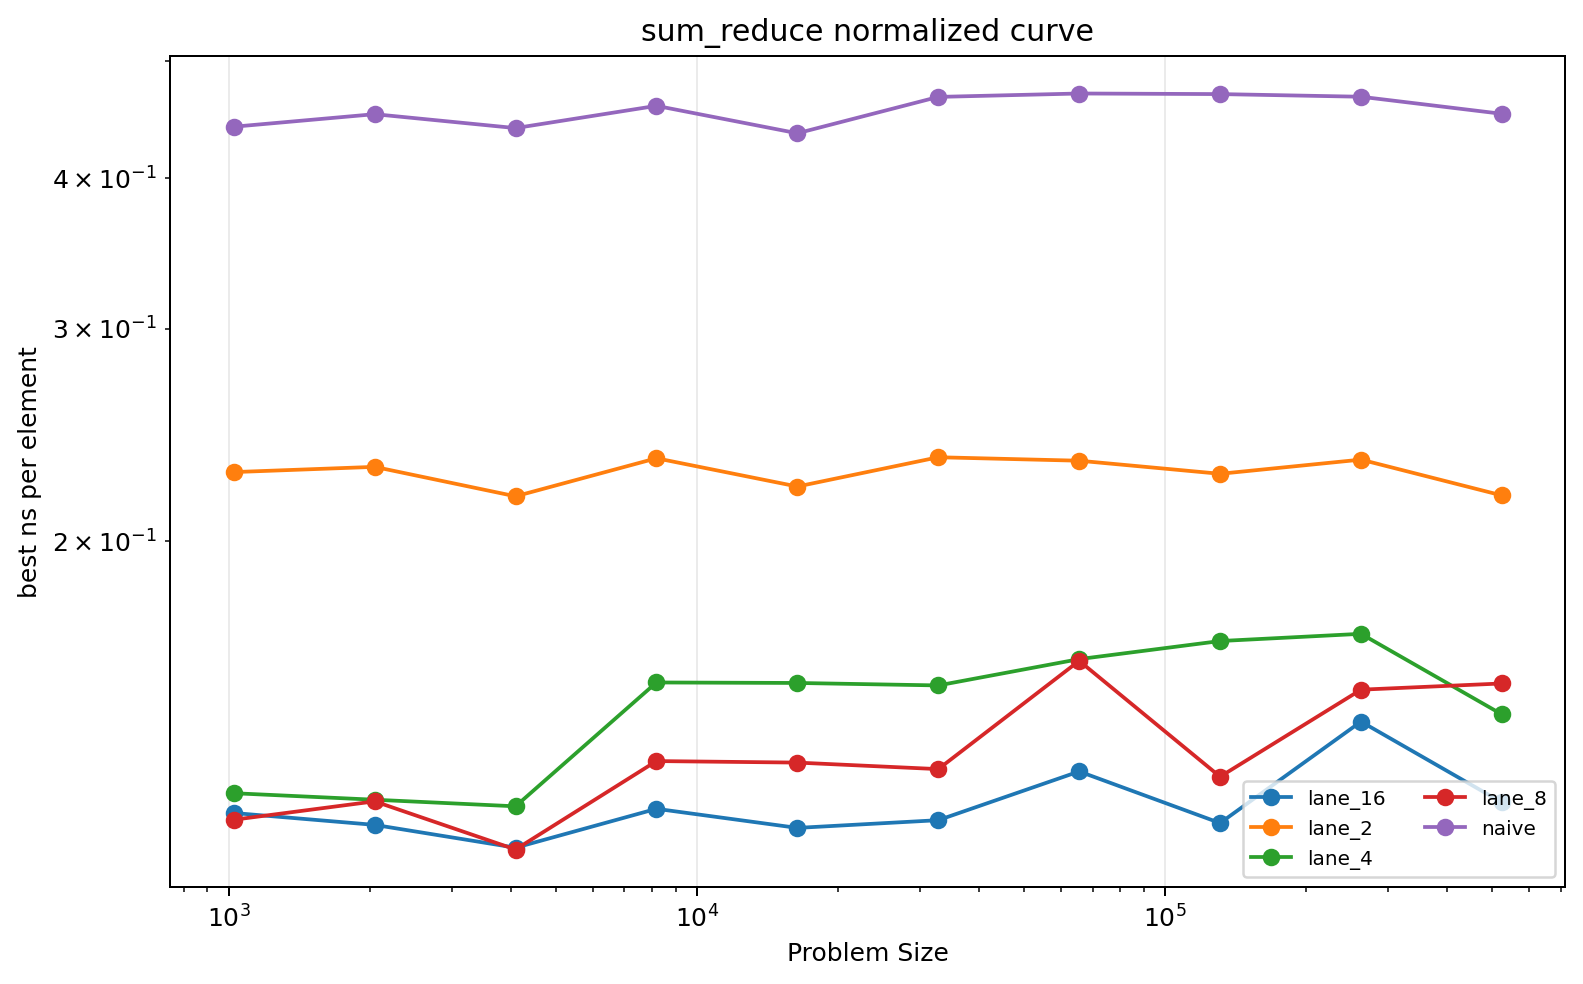
\includegraphics[width=0.82\textwidth]{figures/03_experiments/02_sum_reduce/sum_normalized_curve.png}
\caption{Sum Reduce 归一化耗时曲线（Normalized Runtime Curve）}
\label{fig:sum_normalized_curve}
\end{figure}

\begin{figure}[H]
\centering
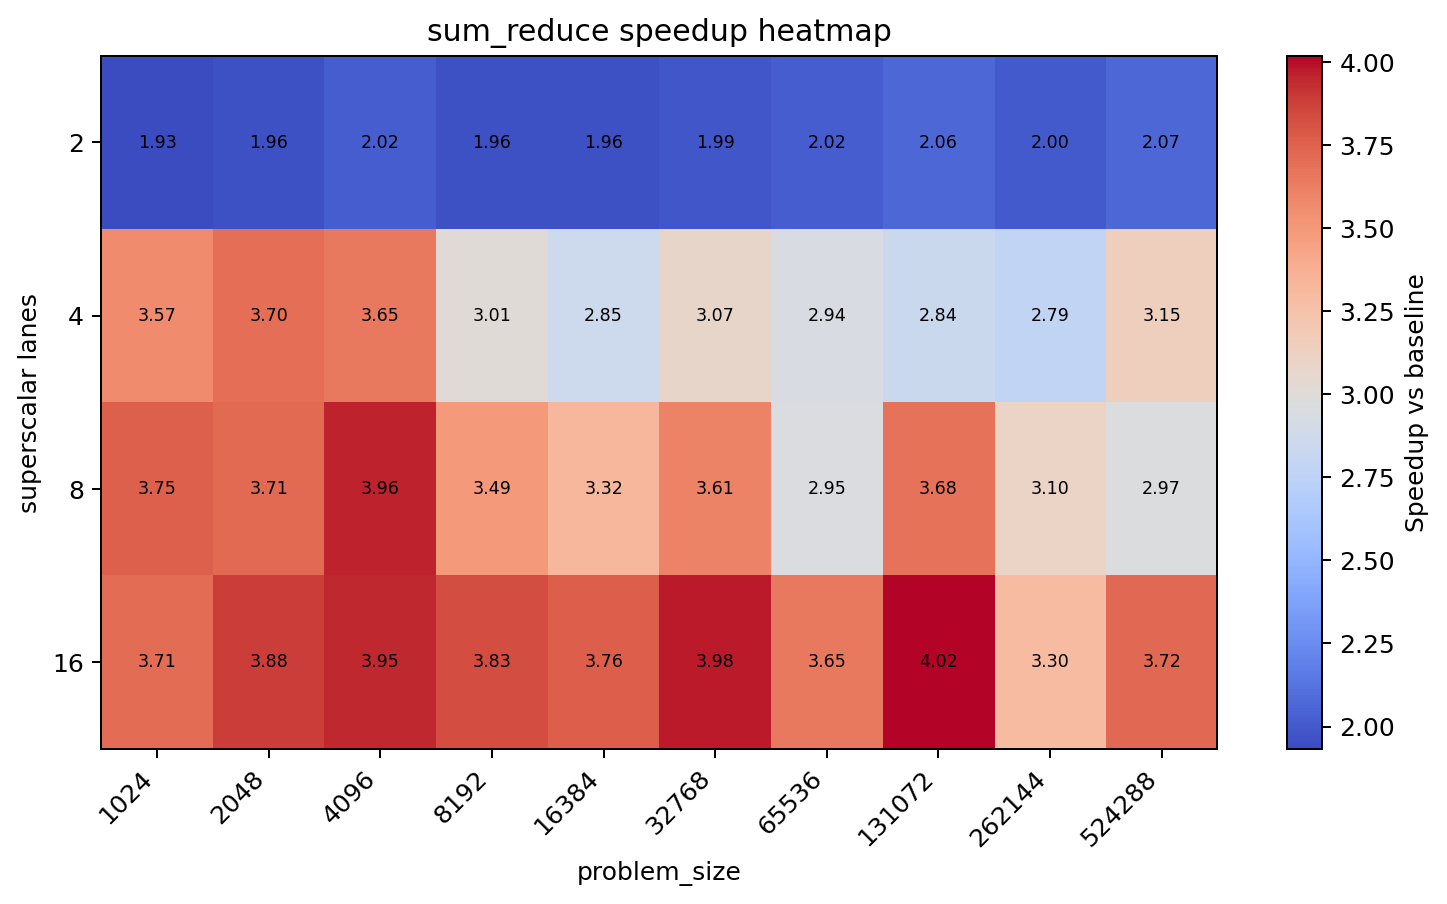
\includegraphics[width=0.82\textwidth]{figures/03_experiments/02_sum_reduce/sum_speedup_heatmap.png}
\caption{Sum Reduce 加速比热力图（Speedup Heatmap）}
\label{fig:sum_speedup_heatmap}
\end{figure}

图 \ref{fig:sum_normalized_curve} 显示，修复后 superscalar 路径在全规模区间均显著优于 naive 基线。图 \ref{fig:sum_speedup_heatmap} 则表明，高收益区域集中在中高 lane 配置，其中 lane=16 在多数规模上表现最稳健。

\begin{table}[H]
\centering
\caption{Sum Reduce 结果汇总}
\label{tab:sum_reduce_after_fix_results}
\small
\begin{tabular}{r r r r r}
\toprule
problem\_size & naive mean(ns) & best superscalar mean(ns) & best lane & speedup \\
\midrule
1024 & 453.385 & 121.875 & 8 & 3.72x \\
2048 & 926.823 & 246.094 & 16 & 3.77x \\
4096 & 1855.208 & 461.198 & 16 & 4.02x \\
8192 & 3799.740 & 983.854 & 16 & 3.86x \\
16384 & 7404.948 & 1918.229 & 16 & 3.86x \\
32768 & 16029.948 & 3860.938 & 16 & 4.15x \\
65536 & 31409.115 & 10675.000 & 8 & 2.94x \\
131072 & 63255.208 & 15786.719 & 16 & 4.01x \\
262144 & 122703.646 & 38325.781 & 16 & 3.20x \\
524288 & 243235.677 & 65128.125 & 16 & 3.73x \\
\bottomrule
\end{tabular}
\end{table}

由表 \ref{tab:sum_reduce_after_fix_results} 可见，修复后最优配置在多数规模上实现约 $3\times$ 到 $4\times$ 的加速，峰值约为 $4.15\times$。该结果与图示趋势一致，说明通过消除实现缺陷并匹配合适并行 lane，可将指令级并行性有效转化为可重复的端到端吞吐提升。